\documentclass[10pt]{beamer}

%%%
% PREAMBLE FOR THIS DOC 
%%%
%https://tex.stackexchange.com/questions/68821/is-it-possible-to-create-a-latex-preamble-header
\usepackage{/Users/miw267/Repos/csci246_spring2025/slides/preambles/beamer_preamble_for_CSCI246}



%%% TRY TO RESHOW TOC AT EACH SECTION START (with current section highlighted)
% Reference: https://tex.stackexchange.com/questions/280436/how-to-highlight-a-specific-section-in-beamer-toc
\newcommand\tocforsect[2]{%
  \begingroup
  \edef\safesection{\thesection}
  \setcounter{section}{#1}
  \tableofcontents[#2,currentsection]
  \setcounter{section}{\safesection}
  \endgroup
}


%%%% HERES HOW TO DO IT CORRECTLY
% FIRST IN .STY FILE, DO
%\usetheme[sectionpage=none]{metropolis}
% THEN AT EACH SECTION DO
%\begin{frame}{Outline}
%  \tableofcontents[currentsection]	
%\end{frame}



%\setbeamertemplate{navigation symbols}{}
%\setbeamertemplate{footline}[frame number]{}


%%%
% DOCUMENT
%%%

\begin{document}

%\maketitle

%% Title page frame
%\begin{frame}
%    \titlepage 
%\end{frame}





\title{02/05/2025: Lists}
\author{CSCI 246: Discrete Structures}
\date{Textbook reference: Sec. 8, Scheinerman}

\begin{frame}
    \titlepage 
\end{frame}


\begin{frame}
\footnotesize 

\begin{mygreenbox}[title=Graded Quiz Pickup]
Quizzes are in the front of the room, grouped into four bins (A-G, H-L, M-R, S-Z) by last name. The quizzes are upside down with your last name on the back. Come find yours before, during, or after class.  Only turn the quiz over if it's yours.
\end{mygreenbox} 
\vfill 

\begin{myredbox}[title=Announcements]

\begin{itemize}
\item Friday's problems quiz will cover \textbf{Boolean Algebra} and \textbf{Induction}.
\item The handwritten scores on Friday's quizzes were presented out of five points TOTAL (2.5 points per problem), but the histograms I showed last class were out of five points per each question.   
\end{itemize}

\end{myredbox}

\vfill 


\begin{myyellowbox}[title=Today's Agenda]
\begin{itemize}
	\item Reading quiz  (5 mins)
	\item Mini-lecture ($\approx$ 20 mins)
	%
	\begin{itemize}
	\footnotesize 
	\item Review induction 
	\end{itemize}
	%
	\item Group exercises ($\approx$ 20 mins)
\end{itemize}

\end{myyellowbox}
\vfill 

\end{frame}




\begin{frame}{Today's Quiz}

\begin{myyellowbox}[title=Logistics Alert]
Please write your last name on the back of the page. 
\end{myyellowbox}

\vfill


 \begin{mygreenbox}[title=Reading Quiz (Lists)]
Five students in our class are randomly selected to form an emergency rock band.  The rock band will have a singer, a guitarist, a bassist, a drummer, and a keyboardist.  How many different rock bands can be formed in this way?  \\

Notes: (1) No student plays more than one instrument (and singing counts as an instrument). (2) If different students play different instruments, it counts as a "different band". (3) Our class has 67 students.
\end{mygreenbox}
\end{frame}



\begin{frame}{Monday's Reading Quiz on Induction}

\begin{myredbox}[title=Scoring rubric]
\begin{tabularx}{\textwidth}{|X|L{1cm}|}
\hline 
\textbf{Description} & \textbf{E.C.} \\
\hline 
Correct and well-written. & +20\% \\
 Good work but some mathematical or writing errors that need addressing. & +15\%\\
Some good intuition (about induction), but there is at least one serious flaw. & +5\%  \\
I don't understand this, but I see that you did work on it. & +0\%  \\
No work is evident.	&+0\% \\
\hline
\end{tabularx}
\end{myredbox}
\end{frame}


\begin{frame}[standout]
Review Induction Group Exercises.
	
\end{frame}




\begin{frame}
\footnotesize
Group 1: bridger.voss,jakob.kominsky,pendleton.johnston\\
Group 2: lucas.jones6,anthony.mann,jacob.ketola\\
Group 3: michael.oswald,lynsey.read,john.fotheringham\\
Group 4: connor.yetter,ryan.barrett2,jonas.zeiler\\
Group 5: sarah.periolat,jacob.ruiz1,william.elder1\\
Group 6: joseph.mergenthaler,matthew.nagel,aaron.loomis\\
Group 7: owen.obrien,kaden.price,erik.moore3\\
Group 8: ethan.johnson18,micaylyn.parker,luke.donaldson1\\
Group 9: jeremiah.mackey,tyler.broesel,joseph.triem\\
Group 10: timothy.true,caitlin.hermanson,jack.fry\\
Group 11: samuel.rollins,nolan.scott1,justice.mosso\\
Group 12: james.brubaker,delaney.rubb,emmeri.grooms\\
Group 13: samuel.hemmen,blake.leone,mason.barnocky\\
Group 14: colter.huber,connor.mizner,yebin.wallace\\
Group 15: conner.reed1,devon.maurer,derek.price4\\
Group 16: griffin.short,adam.wyszynski,carsten.brooks\\
Group 17: carver.wambold,alexander.knutson,tristan.nogacki\\
Group 18: evan.schoening,cameron.wittrock,samuel.mosier\\
Group 19: zeke.baumann,reid.pickert,luka.derry\\
Group 20: julia.larsen,jett.girard,alexander.goetz\\
Group 21: connor.graville,jacob.shepherd1,jada.zorn\\
Group 22: evan.barth,peyton.trigg,peter.buckley1\\\end{frame}


\begin{frame}{Group exercises: Lists}
\footnotesize 

    \begin{minipage}{0.85\textwidth} % Left side (text)
	\begin{enumerate}
	\item I want to create two playlists on my cell phone by downloading from a collection of 500 songs. One playlist is called "Exercise" and the other is called "Relaxing".  I want 20 different songs on each list.  How many different ways can I load songs onto my phone if I allow a song to be on both playlists?  And how many different ways can I load the songs if I want the two lists to have no overlap? 
	\item A padlock has digits 0 through 9 arranged in a circle on its face. A combination for this padlock is four digits long. Because of the internal mechanics of the lock, no pair of consecutive numbers in the combination can be the same or one place apart on the face.  For example, 0-2-7-1 is a valid combination, but neither 0-4-4-7 (repeated digit 4) nor 3-0-9-5 (adjacent digits 0-9) are permitted.  How many combinations are possible?
	\item Four cards are drawn from a standard deck of 52 cards. In how many ways can this be done if the cards are all of different values (e.g., no two 5s or two jacks) and all of different suits?  (For this problem, the order in which the cards are drawn matters, so drawing $A \spadesuit-K \heartsuit - 3 \diamondsuit - 6 \clubsuit$ is not the same as drawing $6 \clubsuit -K \heartsuit - 3 \diamondsuit - A \spadesuit$, even though the same cards are selected.) 
	\item Let $n$ be a positive integer. Prove that $n^2 = (n)_2 + n$ in two different ways: (1) algebraically, and (2) by list counting.
	\end{enumerate}
    \end{minipage}%
    \hfill
    \begin{minipage}{0.15\textwidth} % Right side (image)
        \centering
		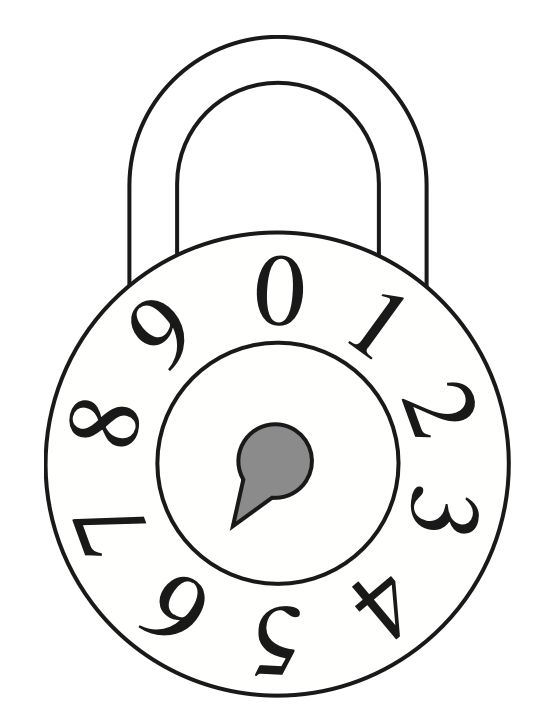
\includegraphics[width=0.9\textwidth]{images/padlock}
    \end{minipage}
    


\vfill 
\centering

\end{frame}


\begin{frame}

To derive the solutions, it may help to apply the theorems below. 

\vfill 

\begin{myyellowbox}[title= \textbf{Multiplication Principle} (Theorem 8.2 from Scheinerman)]
Consider the two-element lists for which there are $n$ choices for the first element, and for each choice of the first element there are $m$ choices for the second element. Then the number of such lists is $nm$.
\end{myyellowbox}
\vfill 

\begin{mygreenbox}[title= Theorem 8.6 from Scheinerman]
The number of lists of length $k$ whose elements are chosen from a pool of $n$ elements 
%
\begin{align*}
= \begin{cases}
 n^k, & \text{if repetitions are permitted} \\
 (n)_k, & \text{if repetitions are forbidden}	
 \end{cases}
\end{align*}
\end{mygreenbox}

	
\end{frame}


\begin{frame}{Solution to \#1}
\small
\textbf{Problem.} I want to create two playlists on my cell phone by downloading from a collection of 500 songs. One playlist is called "Exercise" and the other is called "Relaxing".  I want 20 different songs on each list.  How many different ways can I load songs onto my phone if I allow a song to be on both playlists?  And how many different ways can I load the songs if I want the two lists to have no overlap? 

\vfill 

\textbf{Solution.}
\begin{itemize}
\item[a)] By Theorem 8.6 of Scheinerman, there are $(500)_{20} = 500 \cdot 499 \cdot 498 \cdots 481$ ways to construct either the Exercise playlist, and likewise for the Relaxing playlist.  So applying the multiplication principle to the two types of playlists, the total number of ways to load the songs is $(500)_{20} \cdot (500)_{20}$ (which can be written as $((500)_{20})^2$).
\item[b)] By Theorem 8.6 of Scheinerman, the solution is $(500)_{40} = 500 \cdot 499 \cdot 498 \cdots 461$.  Alternatively, one could argue that there are $(500)_{20}$ ways to construct the first playlist and $(480)_{20}$ ways to construct the second playlist; hence, by the multiplication principle the total number of ways to load the songs is  $(500)_{20} \cdot (480)_{20}$. Note that these two answers are equal; that is  $(500)_{40} = (500)_{20} \cdot (480)_{20}$.
\end{itemize}

%\vfil 
%\textbf{Remark.} We can derive the solution from Theorem 8.6 of Scheinerman 
% 
\end{frame}



\begin{frame}{Solution to \#2}
\textbf{Problem.} A padlock has digits 0 through 9 arranged in a circle on its face. A combination for this padlock is four digits long. Because of the internal mechanics of the lock, no pair of consecutive numbers in the combination can be the same or one place apart on the face.  For example, 0-2-7-1 is a valid combination, but neither 0-4-4-7 (repeated digit 4) nor 3-0-9-5 (adjacent digits 0-9) are permitted.  How many combinations are possible?

\vfill 

\textbf{Solution.}  By the multiplication principle, the total number of solutions is $10 \cdot 7 \cdot 7 \cdot 7$.

\end{frame}


\begin{frame}{Solution to \#3}
\footnotesize 
\textbf{Problem.} Four cards are drawn from a standard deck of 52 cards. In how many ways can this be done if the cards are all of different values (e.g., no two 5s or two jacks) and all of different suits?  (For this problem, the order in which the cards are drawn matters, so drawing $A \spadesuit-K \heartsuit - 3 \diamondsuit - 6 \clubsuit$ is not the same as drawing $6 \clubsuit -K \heartsuit - 3 \diamondsuit - A \spadesuit$, even though the same cards are selected.) 

\vfill 

\textbf{Solution.} The number of ways this can be done is $13 \cdot 4 \cdot 12 \cdot 3 \cdot 11 \cdot 2 \cdot 10 \cdot 1$. By the multiplication principle, the number of choices for the first card is $C_1 \defeq 13 \cdot 4$, since there are 13 values and 4 suits available.  (See the table below.)  After that choice, we cross out one value (column) and one suit (row).  So by the multiplication principle again, the number of choices for the second card is $C_2 \defeq  12 \cdot 3$.  Continuing in this manner, the number of choices for the third card is $C_3 \defeq  11 \cdot 2$ and for the fourth card is $C_4 \defeq  10 \cdot 1$.   Then, applying the multiplication principle again, the number of ways to draw all four cards is $C_1 \cdot C_2 \cdot C_3 \cdot C_4$.


\vfill 

\begin{table}
\centering
\begin{tabular}{c|ccccccccccccc}
\textbf{Suits} & \multicolumn{13}{c}{\textbf{Values}} \\
& A & 2 & 3 & 4 & 5 & 6 & 7 & 8 & 9 & 10 & J & Q & K \\
\hline 
$\spadesuit$ & (A, $\spadesuit$) & (2, $\spadesuit$)  & (3, $\spadesuit$)  &  \multicolumn{9}{c}{$\cdots$}  \\
$\heartsuit$  & (A, $\heartsuit$) &  \multicolumn{12}{c}{$\cdots$} \\
$\diamondsuit$ & (A, $\diamondsuit$) &  \multicolumn{12}{c}{$\cdots$} \\
$\clubsuit$ &  (A, $\clubsuit$) &  \multicolumn{12}{c}{$\cdots$} \\
\end{tabular}
\end{table}



\end{frame}


\begin{frame}{Solution to \#4}
\textbf{Problem.} Let $n$ be a positive integer. Prove that $n^2 = (n)_2 + n$ in two different ways: (1) algebraically, and (2) by list counting.
\vfill 
\textbf{Solution}
\begin{enumerate}
	\item By applying the definition of the falling factorial and doing simple algebra, we see that $(n)_2 +n = n(n-1) +n = n^2 - n + n = n^2$.
	\item We can think of $(n)_2 = n(n-1)$ as the number of lists in a chart with $n$ rows and $n-1$ columns.  Now suppose we add another column.  This gives us $n$ additional lists, making the total number of lists $(n)_2 + n$. But the new chart now has $n$ rows and $n$ columns, so it contains $n \cdot n =n^2$ lists.
\end{enumerate}
\end{frame}

\end{document}
